\def\V{\text{\sc Vrai}\,}
\def\F{\text{\sc Faux}\,}
\def\ite{\text{\sc ite}\,}
%-------------------------------------------------------------------------------
%-------------------------------------------------------------------------------
\chapter{IF-expressions}
%-------------------------------------------------------------------------------
%-------------------------------------------------------------------------------
\thispagestyle{empty}
%-------------------------------------------------------------------------------
%-------------------------------------------------------------------------------
\begin{abstract}
Dans ce T.P. nous allons utiliser un nouveau connecteur logique qui va permettre d'implémenter un algorithme de décision qui reconnaît les tautologie, cet algorithme est différent des tables de vérité classiques. Il nous donnera de plus une réfutation lorsque la proposition n'est pas valide, c'est-à-dire une valuation qui donne la valeur {\bf Faux} lorsqu'on l'applique à la proposition.


On testera la satisfiabilité d'une formule $F$ en appliquant le test à $\neg F$.
\end{abstract}
%-------------------------------------------------------------------------------
%-------------------------------------------------------------------------------
%-------------------------------------------------------------------------------
\section{IF-expressions}
%-------------------------------------------------------------------------------
%-------------------------------------------------------------------------------
%-------------------------------------------------------------------------------
\subsubsection*{Formules classiques}
%-------------------------------------------------------------------------------
%-------------------------------------------------------------------------------

On considère les formules logiques vues en cours.

On ajoute 3 nouveaux symboles.
%-------------------------------------------------------------------------------
\begin{itemize}
\item Les propositions \V et \F. 
Sémantiquement ce sont des constantes qui prennent la valeur {\bf Vrai} ou {\bf Faux} respectivement pour toute valuation.

Pour toute formule $F$, \V est équivalente à $F \lor \neg F$ (resp. à $F \land \neg F$).

Elles seront considérées comme des formules élémentaires, au même titre que les variables.
\item Le connecteur $\rightarrow$.
$F \rightarrow G$ est équivalent à $G \lor \neg F$.

Son but est de permettre des écritures simplifiées.
\end{itemize}
%-------------------------------------------------------------------------------
\smallskip
On représentera les propositions par le type Caml suivant :
%-------------------------------------------------------------------------------
\begin{lstlisting}
type proposition =
  |Var of string
  |Vrai
  |Faux
  |Neg of proposition
  |Donc of proposition * proposition
  |Et of proposition * proposition
  |Ou of proposition * proposition;;
\end{lstlisting}
%-------------------------------------------------------------------------------
%-------------------------------------------------------------------------------
\subsubsection*{IF-expressions}
%-------------------------------------------------------------------------------
%-------------------------------------------------------------------------------
Pour réaliser cet objectif on introduit la notion de \textbf{IF-expression} : 

une IF-expression est soit une variable, soit \V\ ou \F, soit une proposition de la forme $\ite(M, P, Q)$  où $M$, $P$ et $Q$ sont des IF-expression. 

La sémantique d'une IF-expression $\ite(M, P, Q)$ est déterminée récursivement comme 
prenant la valeur de $P$ si $M$ est évaluée à {\bf Vrai} et la valeur de $Q$ sinon. 

Autrement dit $\ite(M, P, Q)$ se traduit par "{\it si M alors P sinon Q}".

ITE est un acronyme pour If Then Else.

On représentera les IF-expressions par le type Caml suivant :
%-------------------------------------------------------------------------------
\begin{lstlisting}
type ifExpr =
  |Var_ite of string
  |Vrai_ite
  |Faux_ite
  |Ite of ifExpr * ifExpr * ifExpr;;
\end{lstlisting}
%-------------------------------------------------------------------------------
%-------------------------------------------------------------------------------
\subsection{Traduction}
%-------------------------------------------------------------------------------
%-------------------------------------------------------------------------------
\begin{Exercise}\it 

Exprimer $\neg P$, $P \land Q$, $P \lor Q$ et $(P \rightarrow Q)$ par des formules ne comportant un seul connecteur $\ite$.
\end{Exercise}
%-------------------------------------------------------------------------------
\begin{Answer} $\neg P\equiv \ite(P,\F,\V)$, 

$P \land Q\equiv \ite(P,Q,\F)$, 

$P \lor Q\equiv \ite(P,\V,Q)$, 

$P \rightarrow Q\equiv \ite(P,Q,\V)$.
\end{Answer}
%-------------------------------------------------------------------------------
%-------------------------------------------------------------------------------
\begin{Exercise}\it 

En déduire une fonction {\tt  prop2if} qui transforme une proposition en une IF-expression équivalente.
\end{Exercise}
%-------------------------------------------------------------------------------
\begin{Answer} 
\begin{lstlisting}
let rec prop2if p =
  match p with
  |Var s     -> Var_ite s
  |Vrai      -> Vrai_ite
  |Faux      -> Faux_ite
  |Neg q     -> Ite (prop2if q, Faux_ite , Vrai_ite)
  |Donc (q,r) -> Ite (prop2if q, prop2if r, Vrai_ite)
  |Et (q,r)  -> Ite (prop2if q, prop2if r, Faux_ite )
  |Ou (q,r)  -> Ite (prop2if q, Vrai_ite, prop2if r);;
\end{lstlisting}
\end{Answer}
%-------------------------------------------------------------------------------
%-------------------------------------------------------------------------------
\begin{Exercise}\it 

Donner les IF-expressions correspondant aux trois propositions suivantes : 
\begin{align*}
  P_1 \ :\ & ( A \land B ) \rightarrow A\\
  P_2 \ :\ & A \rightarrow ( A \land B )\\
  P_3  \ :\ & \bigl(A \rightarrow ( A \rightarrow B )\bigr) \rightarrow B\\
\end{align*}
\end{Exercise}
%-------------------------------------------------------------------------------
\begin{Answer} $P_1 \equiv \ite\bigl(\ite (A,B,\F),A,\V\bigr)$,

$P_2 \equiv \ite(A, \ite(A, B, \F), \V)$,

$P_3 \equiv \ite(\ite(A,\ite(A, B, \V), \V), B, \V)$
\end{Answer}
%-------------------------------------------------------------------------------
%-------------------------------------------------------------------------------
\subsection{Forme normale}
%-------------------------------------------------------------------------------
On dit qu'une IF-expression est \textsc{normale} si elle est 
%-------------------------------------------------------------------------------
\begin{itemize}
\item une variable,
\item \V ou \F
\item ou $\ite(s, P, Q)$ où $s$ est une variable 
et $P$ et $Q$ sont deux IF-expressions normales.
\end{itemize}
%-------------------------------------------------------------------------------
%-------------------------------------------------------------------------------
\begin{Exercise}\it 
Écrire une fonction \type{estNormale : ifExpr -> bool} 

qui teste si une IF-expression est normale.
\end{Exercise}
%-------------------------------------------------------------------------------
\begin{Answer} 
\begin{lstlisting}
let rec estNormale p = 
  match p with
  |Ite (Var_ite _, p, q) -> (estNormale p) || (estNormale q)
  |Ite (_,  _,  _) -> false
  |_ -> true;;
\end{lstlisting}
\end{Answer}
%-------------------------------------------------------------------------------
%-------------------------------------------------------------------------------

\medskip

On considère la fonction $\phi$ définie récursivement par
\begin{itemize}
  \item $\phi(\V)=\phi(\F)=1$
  \item $\phi(s)=1$ pour toute variable $s$
  \item $\phi\bigl(\ite(M,P,Q)\bigr)=\phi(M)\bigl(1+\phi(P)+\phi(Q)\bigr) $
\end{itemize}
%-------------------------------------------------------------------------------
%-------------------------------------------------------------------------------
\begin{Exercise}\it Prouver que les transformations suivantes diminuent la valeur de $\phi$.
\begin{align*}
  \ite(\V,P,Q)\ \rightsquigarrow\  & P\\
  \ite(\F,P,Q)\ \rightsquigarrow\  & Q\\
  \ite(\ite(M,P,Q), R, S)\ \rightsquigarrow\  & \ite\bigl(M, \ite(P, R, S), \ite(Q, R, S)\bigr)
\end{align*}

En déduire toute IF-expression est équivalente à une IF-expression normale. 
\end{Exercise}
%-------------------------------------------------------------------------------
\begin{Answer} Chacune de ces transformation donne une IF-expression équivalente à l'expression initiale.

On a bien $\phi(P) < 1 + \phi(P)+\phi(Q)$, $\phi(Q) < 1 + \phi(P)+\phi(Q)$ et 

$\phi(M)\bigl(1+\phi(P)K + \phi(Q)K\bigr)<  \phi(M)\bigl(1+\phi(P) + \phi(Q)\bigr)K$ avec $K=\bigl(1+\phi(R)+\phi(S)\bigr)$.

Si une If-expression n'est pas normale elle contient une composante de la forme $\ite(M,P,Q)$ avec $M=\V$, $M=\F$ ou $M=\ite(M',P',Q')$.

On peut alors appliquer une des transformations en diminuant strictement la valeur de $\phi$.

Si les transformations ne permettaient jamais d'arriver à une forme normale on aurait une suite de formules équivalentes $M_n$ et la suite des $\bigl(\phi(M_n)\bigr)$ formerait une suite strictement décroissante infinie d'entiers positifs ce qui est impossible.

On parvient donc à une IF-expression normale après un nombre fini de transformations.
\end{Answer}
%-------------------------------------------------------------------------------
%-------------------------------------------------------------------------------
\begin{Exercise}\it 
Écrire une fonction \type{normalise : ifExpr -> ifExpr} 

qui transforme toute IF-expression en une IF-expression normale équivalente.
\end{Exercise}
%-------------------------------------------------------------------------------
\begin{Answer} 
\begin{lstlisting}
let rec normalise prop = 
  match prop with
  |Ite (Var_ite s, p, q) -> Ite (Var_ite s, normalise p, normalise q)
  |Ite (Vrai_ite, p, _) -> normalise p
  |Ite (Faux_ite , _, q) -> normalise q
  |Ite (Ite (m, p, q), r, s) -> normalise (Ite (m, Ite (p, r, s), Ite (q, r, s)))
  |p -> p;;
\end{lstlisting}
\end{Answer}
%-------------------------------------------------------------------------------
%-------------------------------------------------------------------------------
\begin{Exercise}\it Donner les IF-expressions normales correspondant à $P_1$, $P_2$ et $P_3$.
\end{Exercise}
%-------------------------------------------------------------------------------
\begin{Answer} $P_1 \equiv \ite (A, \ite(B, A, \V), \V)$,

$P_2 \equiv \ite (A, \ite (A, B, \F), \V)$,

$P_3 \equiv (A, \ite (A, \ite (B, B, \V), B), B)$.
\end{Answer}
%-------------------------------------------------------------------------------
%-------------------------------------------------------------------------------
%-------------------------------------------------------------------------------
\section{Décision sur les IF-expressions}
%-------------------------------------------------------------------------------
%-------------------------------------------------------------------------------
\subsection{Valuation partielle}
%-------------------------------------------------------------------------------
%-------------------------------------------------------------------------------
On appelle \type{valuation partielle} une fonction des variables dans $\{{\bf Vrai}, {\bf Faux}\}$ dont le domaine est fini. 
On représentera une valuation partielle par une liste d'association :
%-------------------------------------------------------------------------------
\begin{lstlisting}
type valuation = (string * bool) list;;
\end{lstlisting}
%-------------------------------------------------------------------------------
%-------------------------------------------------------------------------------
\begin{Exercise}\it 
Écrire une fonction \type{defini :  string -> valuation -> bool} qui renvoie \type{true} ou \type{false} selon que la valuation partielle est ou non définie pour une variable représentée par une chaîne de caractères.
\end{Exercise}
%-------------------------------------------------------------------------------
\begin{Answer} 

\begin{lstlisting}
let rec defini x v = 
  match v with
  |[] -> false
  |(s, _)::vv -> (s = x) || (defini x vv);;
\end{lstlisting}
\end{Answer}
%-------------------------------------------------------------------------------
%-------------------------------------------------------------------------------
\begin{Exercise}\it 
Écrire une fonction \type{valeur :  string -> valuation -> bool} qui renvoie la valeur prise par une  valuation partielle pour une variable représentée par une chaîne de caractères.
\end{Exercise}
%-------------------------------------------------------------------------------
\begin{Answer} 

\begin{lstlisting}
let rec valeur x v =
  match v with
  |[] -> failwith "non valué"
  |(s,b)::vv ->  if s = x then b else valeur x vv;;
\end{lstlisting}
\end{Answer}
%-------------------------------------------------------------------------------
%-------------------------------------------------------------------------------

\bigskip


Une valuation partielle $\alpha$ définit une valeur booléenne pour toute proposition $P$ dont les variables sont dans le domaine de définition de $\alpha$. On dit alors que $\alpha$ est compatible avec $P$.

On prolonge la notion de tautologie par la notion de $\alpha$-tautologie de la manière suivante :
%-------------------------------------------------------------------------------
\begin{defin}
Une expression $P$ est une $\alpha$-tautologie si elle est vraie pour toutes les valuations partielles qui prolongent $\alpha$ et qui sont compatibles avec $P$.
\end{defin}
%-------------------------------------------------------------------------------
Ainsi $P$ est une tautologie si et seulement si elle est une $\omega$-tautologie où $\omega$ est la valuation partielle de domaine vide.
%-------------------------------------------------------------------------------
%-------------------------------------------------------------------------------
\subsection{Algorithme}
%-------------------------------------------------------------------------------
%-------------------------------------------------------------------------------

Nous allons étudier un algorithme qui détermine si une IF-expression normale $P$ est une $\alpha$-tautologie 
ou, si elle ne l'est pas, détermine une valuation partielle compatible avec $P$, qui prolonge 
$\alpha$ et qui réfute $P$.

Cet algorithme est décrit par les règles suivantes.
%-------------------------------------------------------------------------------
%-------------------------------------------------------------------------------
\begin{enumerate}
\item Si $p$ est \type{True} ou \type{False} le résultat est immédiat.
%-------------------------------------------------------------------------------
%-------------------------------------------------------------------------------
\item Si $p$ est une variable \type{s} alors trois cas se présentent :
%-------------------------------------------------------------------------------
\begin{itemize}
\item si $\alpha(s)$ est défini et vaut {\bf V} alors $P$ est une $\alpha$-tautologie, 
%-------------------------------------------------------------------------------
\item si $\alpha(s)$ est défini et vaut {\bf F} alors $P$ n'est pas une $\alpha$-tautologie, réfutée par $\alpha$,
%-------------------------------------------------------------------------------
\item si $\alpha(s)$ n'est pas défini alors $P$ n'est pas une $\alpha$-tautologie 

et on obtient une réfutation en étendant $\alpha$ par $\alpha(s)={\bf F}$.
\end{itemize}
%-------------------------------------------------------------------------------
%-------------------------------------------------------------------------------
\item  Si $P$ est une IF-expression \type{ite(s, Q, R)} alors
%-------------------------------------------------------------------------------
\begin{itemize}
\item si $\alpha(s)$ est défini et vaut \V

alors $P$ est une $\alpha$-tautologie si et seulement si $Q$ est une $\alpha$-tautologie,
%-------------------------------------------------------------------------------
\item si $\alpha(s)$ est défini et vaut \F

alors $P$ est une $\alpha$-tautologie si et seulement si $R$ est une $\alpha$-tautologie,
%-------------------------------------------------------------------------------
\item si $\alpha(s)$ n'est pas défini alors on définit deux prolongements de $\alpha$, $\alpha_v$ et $\alpha_f$, par $\alpha_v(s) = {\bf V}$ et  $\alpha_f(s)={\bf F}$. $P$ est une $\alpha$ -tautologie si et seulement si $Q$ est une $\alpha_v$-tautologie et $R$ est une $\alpha_f$-tautologie.
\end{itemize}
%-------------------------------------------------------------------------------
\end{enumerate}
%-------------------------------------------------------------------------------
%-------------------------------------------------------------------------------
\begin{Exercise}\it 

Si \type{P = ite(s, Q, R)} n'est pas une $\alpha$-tautologie donner une réfutation dans chacun des 3 cas précédents.
\end{Exercise}
%-------------------------------------------------------------------------------
\begin{Answer} 
\begin{itemize}
\item Si $\alpha(s)={\bf V}$ alors une réfutation de $Q$ est une réfutation de $P$.
\item Si $\alpha(s)={\bf F}$ alors une réfutation de $R$ est une réfutation de $P$.
\item si $\alpha(s)$ n'est pas défini alors une réfutation de $P$ est une réfutation de $Q$ si $Q$ n'est pas une $\alpha_v$-tautologie ou une réfutation de $R$ si $R$ n'est pas une $\alpha_f$-tautologie  .
\end{itemize}
%-------------------------------------------------------------------------------
\end{Answer}
%-------------------------------------------------------------------------------

\bigskip
On définit donc le type suivant pour gérer le résultat de l'algorithme.
%-------------------------------------------------------------------------------
\begin{lstlisting}
type resultat = Tautologie | Refutation of valuation;;
\end{lstlisting}
%-------------------------------------------------------------------------------
%-------------------------------------------------------------------------------
\begin{Exercise}\it 
Écrire une fonction \type{decisionP : valuation -> ifExpr -> resultat} qui décide si une IF-expression normale est une tautologie par rapport à une valuation (partielle) et donne une réfutation si elle ne l'est pas.
\end{Exercise}
%-------------------------------------------------------------------------------
\begin{Answer} On applique l'algorithme
\begin{lstlisting}
let rec decisionP valu prop =
  match prop with
  |Vrai_ite -> Tautologie
  |Faux_ite  -> Refutation valu
  |Var_ite s when defini s valu -> if valeur s valu
                                   then Tautologie
                                   else Refutation valu
  |Var_ite s -> Refutation ((s, false)::valu)
  |Ite (Var s, p, q) when defini s valu  
     -> if valeur s valu 
        then decisionP valu p
        else decisionP valu q)
  |Ite (Var s, p, q) 
     -> let res = decisionP ((s, true)::valu) p in
        if res  = Tautologie
        then decisionP ((s, false)::valu) q
        else res
  |_ -> failwith "ceci ne devrait pas arriver ";;
\end{lstlisting}
\end{Answer}
%-------------------------------------------------------------------------------
%-------------------------------------------------------------------------------
\begin{Exercise}\it
En déduire une fonction \type{decisionIF : ifExpr -> resultat} qui décide si une IF-expression normale est une tautologie et donne une réfutation si elle ne l'est pas.
\end{Exercise}
%-------------------------------------------------------------------------------
\begin{Answer} 
\begin{lstlisting}
let decisionIF p = decisionP [] p;;
\end{lstlisting}
\end{Answer}
%-------------------------------------------------------------------------------
%-------------------------------------------------------------------------------
\begin{Exercise}\it 
Écrire enfin une fonction \type{decision : proposition -> resultat} qui décide si une proposition est une tautologie et donne une réfutation si elle ne l'est pas.
\end{Exercise}
%-------------------------------------------------------------------------------
\begin{Answer} 
\begin{lstlisting}
let decision p = decisionIF (normalise (prop2if p));;
\end{lstlisting}
\end{Answer}
%-------------------------------------------------------------------------------
%-------------------------------------------------------------------------------
\subsection{Applications}
%-------------------------------------------------------------------------------
%-------------------------------------------------------------------------------
\begin{Exercise}\it
Tester les propositions $P_1$, $P_2$ et $P_3$.
\end{Exercise}
%-------------------------------------------------------------------------------
\begin{Answer} $P_1$ est une tautologie,

$P_2$ est réfutée par $A=\V$ et $B=\F$, 

$P_3$ est réfutée par $A=\F$ et $B=\F$.

\newpage
\end{Answer}
%-------------------------------------------------------------------------------
%-------------------------------------------------------------------------------
\subsubsection{Les dahuts}
%-------------------------------------------------------------------------------
\begin{minipage}[b]{0.36\textwidth}
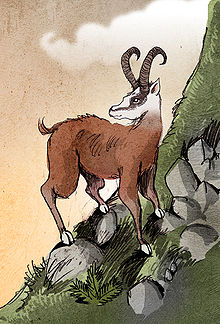
\includegraphics[width=0.8\textwidth]{dahut}
\end{minipage}
\begin{minipage}[b]{0.64\textwidth}
Le dahut est une espèce très rare de bouquetin qui a la particularité d'avoir les deux pattes d'un coté plus courtes que les autres. Il vit donc dans la montagne en ayant toujours le sommet du coté de ses pattes courtes.
 Un dahut est appelé de dextrogyre ou lévogyre selon les cas.
 
 Ils ont d'autres particularités :
%-------------------------------------------------------------------------------
 \begin{itemize}
\item Tout dahut non lévogyre a des rayures noires.
\item Tout dahut qui a des oreilles blanches est lévogyre et vit dans 
les forêts.
\item Tout dahut a des oreilles blanches ou n'a pas de rayures noires.
\item Les dahuts qui vivent dans les forêts ne mangent pas de mulots.
\item Un  dahut mange des mulots si et seulement s'il est lévogyre.
\item Tout dahut lévogyre a des oreilles blanches.
 \end{itemize}
%-------------------------------------------------------------------------------
\end{minipage}

\bigskip
%-------------------------------------------------------------------------------
%-------------------------------------------------------------------------------
\begin{Exercise}\it Prouver que les dahuts n'existent pas.
\end{Exercise}
%-------------------------------------------------------------------------------
\begin{Answer} 
\begin{lstlisting}
let l  = Var "Levogyre";;
let rn = Var "RayuresNoires";;
let ob = Var "OreillesBlanches";;
let f  = Var "vitForet";;
let mm = Var "mangeMulot";;

let d1 = Donc (Neg l, rn);;
let d2 = Ou (ob, Neg rn);;
let d3 = Donc (f, Neg mm);;
let d4 = Et(Donc (mm, l), Donc (l, mm));;
let d5 = Donc (ob, Et (l, f));;
let d6 = Donc (l, ob);;

let p = Neg (Et (Et (Et (d1, d2), Et (d3, d4)), Et (d5, d6)));;
\end{lstlisting}
$p$ est une tautologie donc les conditions donnent une contradiction.
\end{Answer}
%-------------------------------------------------------------------------------
%-------------------------------------------------------------------------------
\subsubsection{La princesse}
%-------------------------------------------------------------------------------
Un chevalier doit partir délivrer des princesses. Arrivé à une intersection, il a le choix entre trois chemins, chacun précédé d'un panneau. Le gardien des lieux lui déclare : 

"{\it Parmi ces trois chemins, l'un mène à une princesse, et son panneau dit la vérité. 

Quant aux deux autres, ils aboutissent à une mort certaine. 

Au moins l'un des panneaux ment.}"

Voici ce qui est écrit à l'entrée de chaque chemin :
%-------------------------------------------------------------------------------
\begin{itemize}
\item Le deuxième chemin mène à une mort certaine.
\item Ce chemin mène à une mort certaine.
\item Le premier chemin mène à une mort certaine.
\end{itemize}
%-------------------------------------------------------------------------------
\begin{Exercise}\it Comment délivrer la princesse ?
\end{Exercise}
%-------------------------------------------------------------------------------
\begin{Answer} 
\begin{lstlisting}
let p1 = Var "Princesse en 1";;
let p2 = Var "Princesse en 2";;
let p3 = Var "Princesse en 3";;

let e1 = Neg p2;;
let e2 = Neg p2;;
let e3 = Neg p1;;

let o1 = Et(Et (p1, e1), Et (Neg p2, Neg p3));;
let o2 = Et(Et (p2, e2), Et (Neg p3, Neg p1));;
let o3 = Et(Et (p3, e3), Et (Neg p1, Neg p2));;

let test = Neg (Ou (Ou (o1, o2), o3));;

decision test;;

Refutation ["Princesse en 3", false; "Princesse en 2", false; 
            "Princesse en 1", true]
\end{lstlisting}
\end{Answer}
%-------------------------------------------------------------------------------
\newpage
%-------------------------------------------------------------------------------
%-------------------------------------------------------------------------------




